\chapter{Boletín B - Problemas resueltos}
%===================
% Boletín B. Problema 3
%===================
\begin{problema}[Distribuciones de carga y factores de forma en $^{11}\text{Be}$]
Calcular el radio cuadrático medio, $a = \sqrt{\langle r^2 \rangle}$, y el factor de forma, $F(q^2)$, para las siguientes distribuciones de carga:
\begin{enumerate}[label=\alph*.-]
    \item $\rho(r) = \rho_0 e^{-r/\alpha}$
    \item $\rho(r) = \begin{cases} \rho_0 & r \le R \\ 0 & r > R \end{cases}$
\end{enumerate}
Comparar las secciones eficaces predichas por ambas distribuciones para la dispersión (\textit{scattering}) de electrones con una energía $E = 183 \MeV$ sobre $^{11}\text{Be}$, suponiendo el mismo valor del radio cuadrático medio en ambos casos. Calcular dicha relación para ángulos de dispersión $\theta = \pi$ y $\theta = \pi/2$.

\tcblower

\subsubsection*{Apartado a: Distribución exponencial}

Consideremos en primer lugar la densidad de carga continua dada por una exponencial decreciente $\rho(r) = \rho_0 e^{-r/\alpha}$, donde $\alpha$ representa la longitud característica del alcance espacial de la carga.

\paragraph{1. Normalización y radio cuadrático medio}
Para determinar la constante de normalización $\rho_0$, imponemos que la carga total de la distribución sea la unidad:
\begin{equation}
    \int \rho(r) \, d^3r = 4\pi \rho_0 \int_0^\infty r^2 e^{-r/\alpha} \, dr = 1
\end{equation}
Para evaluar estas integrales radiales empleamos la definición de la función Gamma o la propiedad de las integrales exponenciales de la forma:
\begin{equation}
    I_n(\alpha) = \int_0^\infty r^n e^{-r/\alpha} \, dr = n! \, \alpha^{n+1}
\end{equation}
Sustituyendo $n = 2$:
\begin{equation}
    4\pi \rho_0 (2! \, \alpha^3) = 8\pi \rho_0 \alpha^3 = 1 \implies \rho_0 = \frac{1}{8\pi \alpha^3}
\end{equation}

A continuación, calculamos el valor medio del radio al cuadrado $\langle r^2 \rangle$:
\begin{equation}
    \langle r^2 \rangle = \int r^2 \rho(r) \, d^3r = 4\pi \rho_0 \int_0^\infty r^4 e^{-r/\alpha} \, dr = 4\pi \rho_0 (4! \, \alpha^5) = 96\pi \rho_0 \alpha^5
\end{equation}
Sustituyendo la constante de normalización $\rho_0 = \frac{1}{8\pi \alpha^3}$:
\begin{equation}
    \langle r^2 \rangle = \frac{96\pi \alpha^5}{8\pi \alpha^3} = 12 \alpha^2
\end{equation}
Por tanto, el radio cuadrático medio $a$ resulta:
\begin{equation}
    a = \sqrt{\langle r^2 \rangle} = 2\sqrt{3} \, \alpha
\end{equation}

\paragraph{2. Cálculo del factor de forma $F(q)$}
Para una distribución esféricamente simétrica, el factor de forma viene dado por la transformada de Fourier tridimensional:
\begin{equation}
    F(q) = \frac{4\pi}{q} \int_0^\infty r \sin(qr) \rho(r) \, dr = \frac{4\pi \rho_0}{q} \int_0^\infty r \sin(qr) e^{-r/\alpha} \, dr
\end{equation}
Consideremos la integral conocida de Laplace:
\begin{equation}
    J(\beta) = \int_0^\infty e^{-\beta r} \sin(qr) \, dr = \frac{q}{\beta^2 + q^2} \quad \text{con } \beta = \frac{1}{\alpha}
\end{equation}
Derivando con respecto a $\beta$ bajo el signo integral:
\begin{equation}
    \int_0^\infty r e^{-\beta r} \sin(qr) \, dr = -\frac{\partial J}{\partial \beta} = -\frac{\partial}{\partial \beta} \left( \frac{q}{\beta^2 + q^2} \right) = \frac{2\beta q}{(\beta^2 + q^2)^2}
\end{equation}
Sustituyendo esta integral en la expresión de $F(q)$:
\begin{equation}
    F(q) = \frac{4\pi \rho_0}{q} \cdot \frac{2(1/\alpha)q}{\left( (1/\alpha)^2 + q^2 \right)^2} = \frac{8\pi \rho_0 \alpha^3}{\left( 1 + \alpha^2 q^2 \right)^2}
\end{equation}
Aprovechando la condición de normalización $8\pi \rho_0 \alpha^3 = 1$, obtenemos el factor de forma difusivo o de dipolo:
\begin{concepto}[Factor de forma exponencial]
\begin{equation}
    F_a(q) = \frac{1}{\left( 1 + \alpha^2 q^2 \right)^2}
\end{equation}
\end{concepto}

\paragraph{3. Verificación mediante desarrollo a bajo momento transferido}
A bajas transferencias de momento ($q \to 0$), todo factor de forma admite el desarrollo en serie de Taylor:
\begin{equation}
    F(q) = 1 - \frac{1}{6} \langle r^2 \rangle q^2 + \mathcal{O}(q^4)
\end{equation}
Desarrollando $F_a(q)$ mediante la serie binomial $(1 + x)^{-2} = 1 - 2x + \mathcal{O}(x^2)$ con $x = \alpha^2 q^2$:
\begin{equation}
    F_a(q) = 1 - 2\alpha^2 q^2 + \mathcal{O}(q^4)
\end{equation}
Igualando los coeficientes del término $q^2$:
\begin{equation}
    -\frac{1}{6} \langle r^2 \rangle = -2\alpha^2 \implies \langle r^2 \rangle = 12\alpha^2
\end{equation}
lo que confirma plenamente la consistencia del resultado obtenido.

\begin{center}
  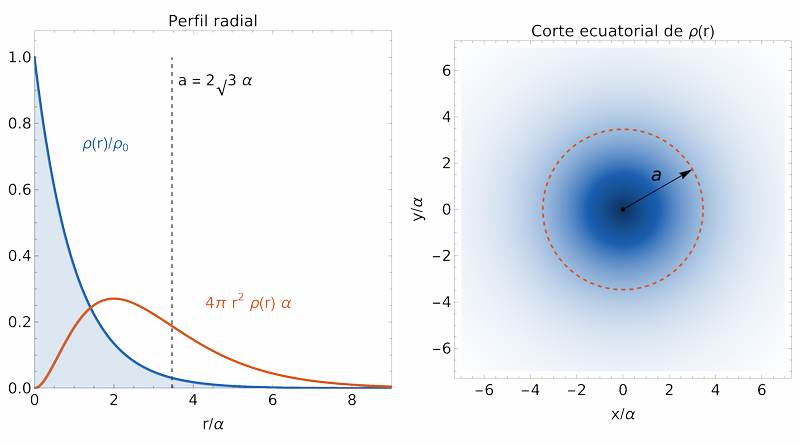
\includegraphics[width=0.6\textwidth]{imagenes/tema2/B2_P3_a.png}
  \captionof{figure}{Representación esquemática de la densidad espacial de carga exponencial.}
  \label{fig:rho_exponencial}
\end{center}

\subsubsection*{Apartado b: Distribución uniforme de esfera dura}

Estudiemos ahora la distribución de densidad constante contenida en una esfera de radio $R$:
\begin{equation}
    \rho(r) = \begin{cases} \rho_0 & r \le R \\ 0 & r > R \end{cases}
\end{equation}

\paragraph{1. Normalización y radio cuadrático medio}
Imponiendo la normalización de la carga sobre el volumen de la esfera:
\begin{equation}
    \int \rho(r) \, d^3r = 4\pi \rho_0 \int_0^R r^2 \, dr = \frac{4}{3}\pi \rho_0 R^3 = 1 \implies \rho_0 = \frac{3}{4\pi R^3}
\end{equation}
Calculamos el radio cuadrático medio $\langle r^2 \rangle$:
\begin{equation}
    \langle r^2 \rangle = 4\pi \rho_0 \int_0^R r^4 \, dr = 4\pi \rho_0 \frac{R^5}{5} = 4\pi \left( \frac{3}{4\pi R^3} \right) \frac{R^5}{5} = \frac{3}{5} R^2
\end{equation}
Por consiguiente, el radio cuadrático medio de la esfera dura es:
\begin{equation}
    a = \sqrt{\langle r^2 \rangle} = \sqrt{\frac{3}{5}} \, R
\end{equation}

\paragraph{2. Cálculo del factor de forma $F(q)$}
Integrando en el dominio acotado $[0, R]$:
\begin{equation}
    F_b(q) = \frac{4\pi \rho_0}{q} \int_0^R r \sin(qr) \, dr
\end{equation}
Integrando por partes con $u = r \implies du = dr$ y $dv = \sin(qr)dr \implies v = -\frac{\cos(qr)}{q}$:
\begin{align}
    \int_0^R r \sin(qr) \, dr &= \left[ -\frac{r \cos(qr)}{q} \right]_0^R + \frac{1}{q} \int_0^R \cos(qr) \, dr \nonumber \\
    &= -\frac{R \cos(qR)}{q} + \frac{\sin(qR)}{q^2} = \frac{\sin(qR) - qR\cos(qR)}{q^2}
\end{align}
Sustituyendo $\rho_0 = \frac{3}{4\pi R^3}$:
\begin{concepto}[Factor de forma de esfera dura]
\begin{equation}
    F_b(q) = \frac{4\pi}{q} \left( \frac{3}{4\pi R^3} \right) \frac{\sin(qR) - qR\cos(qR)}{q^2} = \frac{3}{(qR)^3} \left[ \sin(qR) - qR\cos(qR) \right]
\end{equation}
\end{concepto}

\paragraph{3. Verificación a bajos momentos transferidos}
Desarrollando las funciones trigonométricas en serie de Taylor alrededor de $x = qR \to 0$:
\begin{align}
    \sin(x) &= x - \frac{x^3}{6} + \frac{x^5}{120} - \mathcal{O}(x^7) \\
    x\cos(x) &= x \left( 1 - \frac{x^2}{2} + \frac{x^4}{24} - \mathcal{O}(x^6) \right) = x - \frac{x^3}{2} + \frac{x^5}{24} - \mathcal{O}(x^7)
\end{align}
Restando ambas expresiones:
\begin{equation}
    \sin(x) - x\cos(x) = \left( \frac{1}{2} - \frac{1}{6} \right) x^3 + \left( \frac{1}{120} - \frac{1}{24} \right) x^5 + \dots = \frac{1}{3} x^3 - \frac{1}{30} x^5 + \mathcal{O}(x^7)
\end{equation}
Sustituyendo en $F_b(q)$:
\begin{equation}
    F_b(q) = \frac{3}{x^3} \left( \frac{1}{3} x^3 - \frac{1}{30} x^5 + \dots \right) = 1 - \frac{1}{10} (qR)^2 + \mathcal{O}(q^4)
\end{equation}
Comparando con $1 - \frac{1}{6} \langle r^2 \rangle q^2$:
\begin{equation}
    -\frac{1}{6} \langle r^2 \rangle = -\frac{1}{10} R^2 \implies \langle r^2 \rangle = \frac{6}{10} R^2 = \frac{3}{5} R^2
\end{equation}

\begin{center}
  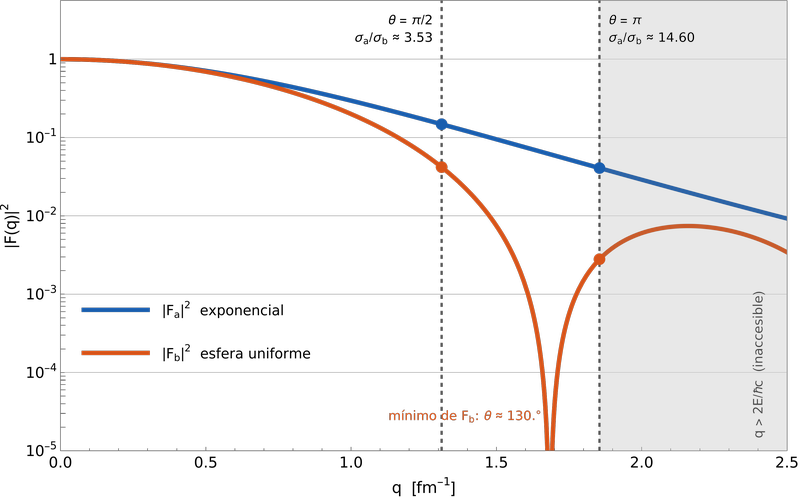
\includegraphics[width=0.6\textwidth]{imagenes/tema2/B2_P3_b.png}
  \captionof{figure}{Comparación de los factores de forma cuadráticos entre la distribución exponencial y la esfera uniforme.}
  \label{fig:factores_forma_comparacion}
\end{center}

\subsubsection*{Apartado c: Comparación de secciones eficaces en $^{11}\text{Be}$}

Nos proponemos comparar el cociente entre las secciones eficaces diferenciales predichas por ambos modelos:
\begin{equation}
    \frac{\left( \frac{d\sigma}{d\Omega} \right)_a}{\left( \frac{d\sigma}{d\Omega} \right)_b} = \frac{|F_a(q)|^2}{|F_b(q)|^2}
\end{equation}
para la dispersión de electrones de $E = 183 \MeV$ sobre un núcleo de $^{11}\text{Be}$ ($A = 11$), imponiendo la igualdad del radio cuadrático medio $\langle r^2 \rangle_a = \langle r^2 \rangle_b$:
\begin{equation}
    12 \alpha^2 = \frac{3}{5} R^2 \implies R = \sqrt{20} \, \alpha = 2\sqrt{5} \, \alpha \approx 4.4721 \, \alpha
\end{equation}

\paragraph{1. Cinematica y transferencia de momento}
Dado que $E = 183 \MeV \gg m_e c^2 = 0.511 \MeV$, el electrón se comporta de forma ultrarrelativista ($p c \approx E$). La transferencia de momento $q$ en términos del ángulo de dispersión $\theta$ satisface:
\begin{equation}
    q = \frac{2p}{\hbar} \sin(\theta/2) \approx \frac{2E}{\hbar c} \sin(\theta/2)
\end{equation}
Utilizando la constante de conversión $\hbar c = 197.327 \MeV \cdot \fm$:
\begin{equation}
    \frac{2E}{\hbar c} = \frac{2 \times 183 \MeV}{197.327 \MeV \cdot \fm} \approx 1.8548 \fm^{-1}
\end{equation}

Para el núcleo de $^{11}\text{Be}$ ($A = 11$), estimamos el radio equivalente de esfera uniforme mediante la parametrización nuclear estándar $R = 1.2 A^{1/3} \fm$:
\begin{equation}
    R = 1.2 \times (11)^{1/3} \fm \approx 1.2 \times 2.2240 \fm \approx 2.6688 \fm
\end{equation}
A partir de la equivalencia de radios cuadráticos medios:
\begin{equation}
    \alpha = \frac{R}{\sqrt{20}} = \frac{2.6688 \fm}{4.4721} \approx 0.5968 \fm
\end{equation}

\paragraph{2. Evaluación para $\theta = \pi$ ($180^\circ$)}
Para retrodispersión ($\theta = \pi$), tenemos $\sin(\theta/2) = \sin(\pi/2) = 1$:
\begin{equation}
    q(\pi) = 1.8548 \fm^{-1}
\end{equation}
Los productos adimensionales para cada factor de forma valen:
\begin{align}
    x = qR &= 1.8548 \times 2.6688 \approx 4.950 \text{ rad} \\
    \alpha q &= 0.5968 \times 1.8548 \approx 1.107
\end{align}

Evaluamos los factores de forma:
\begin{align}
    F_a(q) &= \frac{1}{(1 + 1.107^2)^2} = \frac{1}{(1 + 1.2254)^2} = \frac{1}{4.952} \approx 0.2019 \\
    F_b(q) &= \frac{3}{(4.950)^3} \left[ \sin(4.950) - 4.950 \cos(4.950) \right] \nonumber \\
    &\approx \frac{3}{121.287} \left[ -0.9701 - 4.950 \times (0.2427) \right] \nonumber \\
    &= \frac{3}{121.287} \left[ -0.9701 - 1.2014 \right] \approx -0.0537
\end{align}

El cociente de secciones eficaces resulta:
\begin{observacion}[Relación de secciones eficaces a $\theta = \pi$]
\begin{equation}
    \left. \frac{(d\sigma/d\Omega)_a}{(d\sigma/d\Omega)_b} \right|_{\theta = \pi} = \left| \frac{F_a(q)}{F_b(q)} \right|^2 = \left| \frac{0.2019}{-0.0537} \right|^2 \approx (3.7597)^2 \approx 14.13
\end{equation}
\end{observacion}

\paragraph{3. Evaluación para $\theta = \pi/2$ ($90^\circ$)}
Para un ángulo de dispersión recto, $\sin(\theta/2) = \sin(\pi/4) = 1/\sqrt{2} \approx 0.7071$:
\begin{equation}
    q(\pi/2) = 1.8548 \times 0.7071 \approx 1.3115 \fm^{-1}
\end{equation}
Los productos adimensionales valen:
\begin{align}
    x = qR &= 1.3115 \times 2.6688 \approx 3.500 \text{ rad} \\
    \alpha q &= 0.5968 \times 1.3115 \approx 0.7827
\end{align}

Evaluamos los factores de forma:
\begin{align}
    F_a(q) &= \frac{1}{(1 + 0.7827^2)^2} = \frac{1}{(1 + 0.6126)^2} = \frac{1}{2.600} \approx 0.3846 \\
    F_b(q) &= \frac{3}{(3.500)^3} \left[ \sin(3.500) - 3.500 \cos(3.500) \right] \nonumber \\
    &\approx \frac{3}{42.875} \left[ -0.3508 - 3.500 \times (-0.9365) \right] \nonumber \\
    &= \frac{3}{42.875} \left[ -0.3508 + 3.2778 \right] \approx 0.2048
\end{align}

El cociente de secciones eficaces resulta:
\begin{observacion}[Relación de secciones eficaces a $\theta = \pi/2$]
\begin{equation}
    \left. \frac{(d\sigma/d\Omega)_a}{(d\sigma/d\Omega)_b} \right|_{\theta = \pi/2} = \left| \frac{F_a(q)}{F_b(q)} \right|^2 = \left| \frac{0.3846}{0.2048} \right|^2 \approx (1.8779)^2 \approx 3.53
\end{equation}
\end{observacion}
\end{problema}